\section{Kodo-python}

\subsection{Exercise 0:}
\begin{figure}[H]
    \centering
    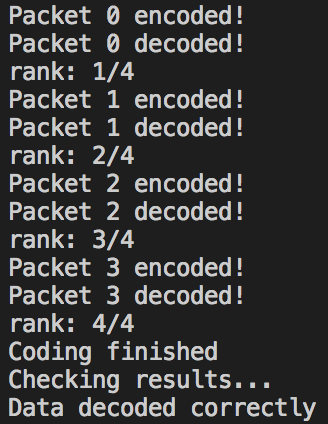
\includegraphics[width=0.2\textwidth]{figures/KodoPython/encode_decode.png}
    \caption{Encode and Decode}
    \label{fig:encode_decode}
\end{figure}

\subsection{Exercise 1:}
\begin{figure}[H]
    \centering
    \begin{subfigure}{.49\textwidth}
        \centering
        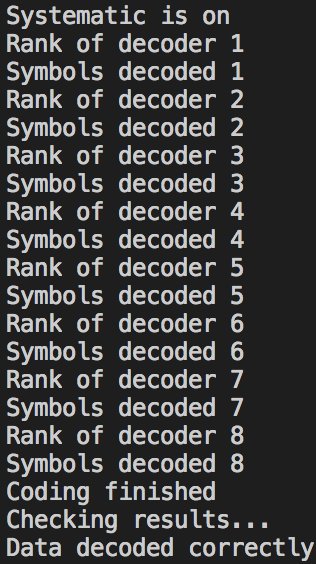
\includegraphics[width=0.4\textwidth]{figures/KodoPython/systematic_on.png}
        \caption{Systematic On}
        \label{fig:systematic_on}
    \end{subfigure}
    \begin{subfigure}{.5\textwidth}
        \centering
        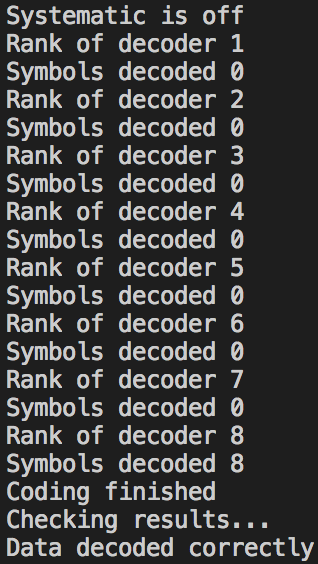
\includegraphics[width=0.4\textwidth]{figures/KodoPython/systematic_off.png}
        \caption{Systematic Off}
        \label{fig:systematic_off}
    \end{subfigure}
    \caption{Systematic On/Off}
    \label{fig:systematic_on_off}
\end{figure}
\textbf{Questions}
\begin{enumerate}
    \item \textit{Identify how many packets the encoder must generate, for the decoder to decode the data, with systematic mode ON and OFF.}\\ 
    Systematic mode on requires only 1 package to decode. The encoder sends the uncoded symbols, when getting a previously uncoded symbol\\
    Systematic mode off requires all packages to decode. The decoder must figure out how to decode the symbols itself.\\
    \textit{ - Do you need to increase the amount of coded packages generate to decode the data with systematic mode OFF?}\\
    YES! See above
    \item \textit{Identify if changes in g and k affect the number of packages generated. Note down your configurations for g and k.}\\
    The number of packages equals g.
    \item \textit{Based, on your knowledge of RLNC, Storage Systems, and Systematic Mode, is systematic mode a beneficial thing or not? In either case argue why.}\\
    It depends on the requirements for the system. It's a trade-off between network traffic and computation time.
\end{enumerate}

\subsection{Exercise 2:}
We have altered the setup a bit, for every value of g, we have tested with k=8...131072.

\begin{figure}[H]
    \centering
    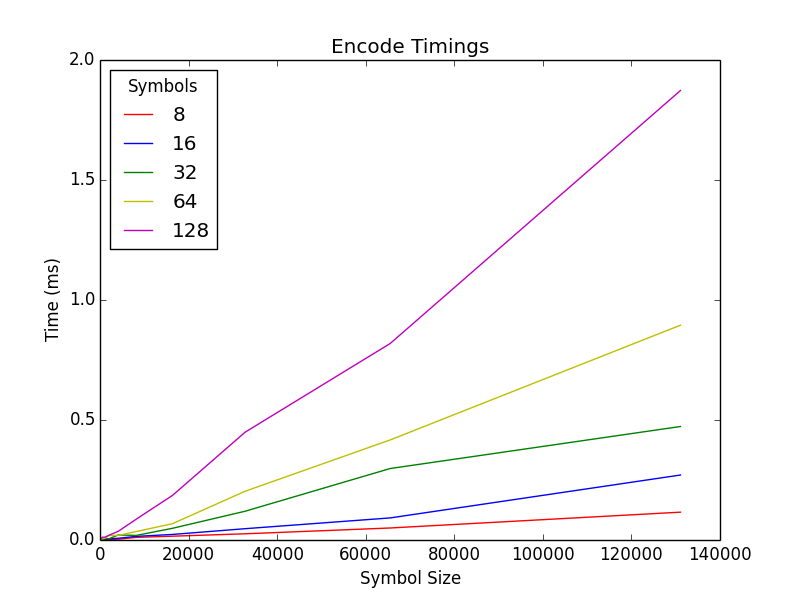
\includegraphics[width=0.7\textwidth]{figures/KodoPython/encode_timings.png}
    \caption{Encode Timings}
    \label{fig:encode_timings}
\end{figure}
\begin{figure}[H]
    \centering
    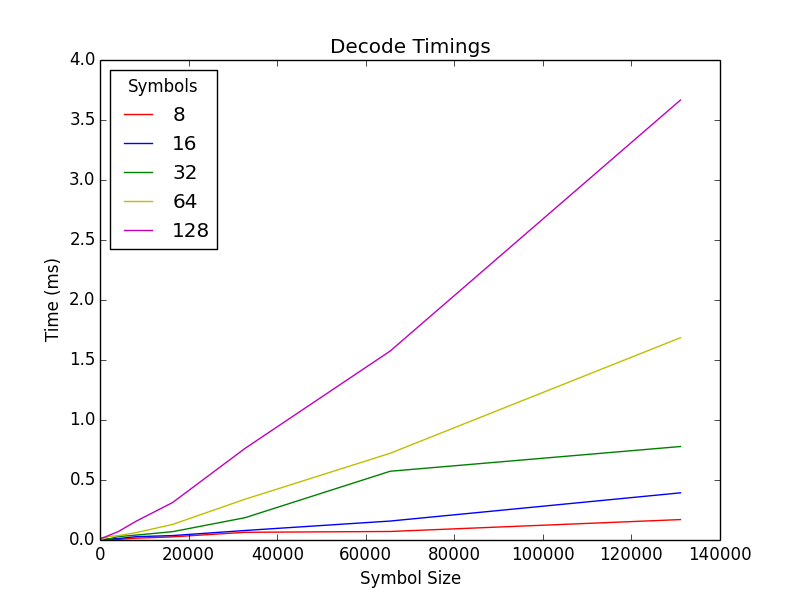
\includegraphics[width=0.7\textwidth]{figures/KodoPython/decode_timings.png}
    \caption{Encode Timings}
    \label{fig:decode_timings}
\end{figure}

The test shows that when g increase with a factor of 2 so does the time of computation.
For higher values of g the bigger impact k has on the computation time, for both encoding and decoding. 

\subsection{Exercise 3:}
Using the supplied Python and image, we have answered the following quiestions:
\begin{enumerate}
    \item \textit{How many clouds can you take down before it becomes impossible to decode the image.}\\
    Our setup: g=128, k=1024, 5 redundancy and 20 clouds.
    We vary the loss percentage in increments of 10\% on see losses from 60\% and upwards.
    \item \textit{Does the configuration for g and k effect the above. Choose your own g and k.}\\
    \begin{table}[H]
        \begin{tabularx}{\textwidth}{|Y|Y|Y|Y|}
            \hline
            \cellcolor{gray}g & \cellcolor{gray}k & \cellcolor{gray}50\% Loss & \cellcolor{gray}60\% Loss \\\hline
            \cellcolor{lightgray}64 & \cellcolor{lightgray}1024 & \textcolor{red}{False}& \textcolor{red}{False}\\\hline
            \cellcolor{lightgray}64 & \cellcolor{lightgray}2048 & \textcolor{green}{True} & \textcolor{red}{False}\\\hline
            \cellcolor{lightgray}64 & \cellcolor{lightgray}4096 & \textcolor{green}{True} & \textcolor{green}{True}\\\hline
            \cellcolor{lightgray}64 & \cellcolor{lightgray}8192 & \textcolor{green}{True} & \textcolor{green}{True}\\\hline
            \cellcolor{lightgray}64 & \cellcolor{lightgray}16384 & \textcolor{green}{True} & \textcolor{green}{True}\\\hline
            \cellcolor{lightgray}128 & \cellcolor{lightgray}1024 & \textcolor{green}{True} & \textcolor{red}{False}\\\hline
            \cellcolor{lightgray}128 & \cellcolor{lightgray}2048 & \textcolor{green}{True} & \textcolor{green}{True}\\\hline
            \cellcolor{lightgray}128 & \cellcolor{lightgray}2096 & \textcolor{green}{True} & \textcolor{green}{True}\\\hline
            \cellcolor{lightgray}128 & \cellcolor{lightgray}8192 & \textcolor{green}{True} & \textcolor{green}{True}\\\hline
            \cellcolor{lightgray}128 & \cellcolor{lightgray}16384 & \textcolor{green}{True} & \textcolor{green}{True}\\\hline
        \end{tabularx}
        \caption{Picture recreation success}
        \label{tab:Exercise3}
    \end{table}

    \item \textit{Reflect on what you observe}\\
    
\end{enumerate}




\subsection{Exercise 4:}
\underline{\textit{Why RLNC should/shouldn't be used in distributed storage, and if you see an alternative:}}\\
First and foremost RLNC can be used to provide reliability in cloud setups. Our setup showed the critical point for
fault tolerance is above 50\%, which is descent enough. 
However, we have only tested when it's critical   

\pagebreak